\section{Results and evaluation}

By extracting the vendors information of both access point and station in all three regions, Figure 1 shows the histogram of numbers of devices using corresponding vendors in three regions. Because a large number of vendors while sniffing only have one or two devices, if all displayed in chart the chart will be long. Thus in the histogram as shown in figure 1, all of this kind of vendors are classified into "others" vendor type but they are still taken into account when the nationality of the vendors is counted later.
\newline
Figures (a),(c),(e) from figure 1 show three different distributions of the Access Points' vendor types. On campus, Cisco's amount accounts for the vast majority, more than the other operators combined. That's easy to explain because TU Delft are all covered by Access Points provided by Cisco. And in the other two areas, the vendor types that could not be found in the Wireshark manufacturer database are much more than others. Besides the "not found" part, TP-Link, Compal, Arcadyan, ARRIS and zte are also the people's preferable choices.
\newline
As for the distribution of stations in these three areas,  according to online data from statcounter global stats which is shown in figure 2, Apple ranks first in the Netherlands, followed by Huawei and Xiaomi. Compared with figures (b),(d),(f), the experimental data included additional group of devices using vendors of Google, Inc. which accounted for a large proportion in all three regions. Apart from the unknown vendors, the arrangement of other vendors is basically similar the the data on the website. It is also clear from the figure that Apple, Google and Intel all have a large proportion in all three regions which is similar to the situation of people using devices in daily life. The difference is that the ratio of Apples vendor is higher in places like campus where there are more young people, but not in places like Hendrick where there are more middle-aged or even older people.

\newpage

\begin{figure}[H]
    \centering
    \subfigure[Access points on campus]{
        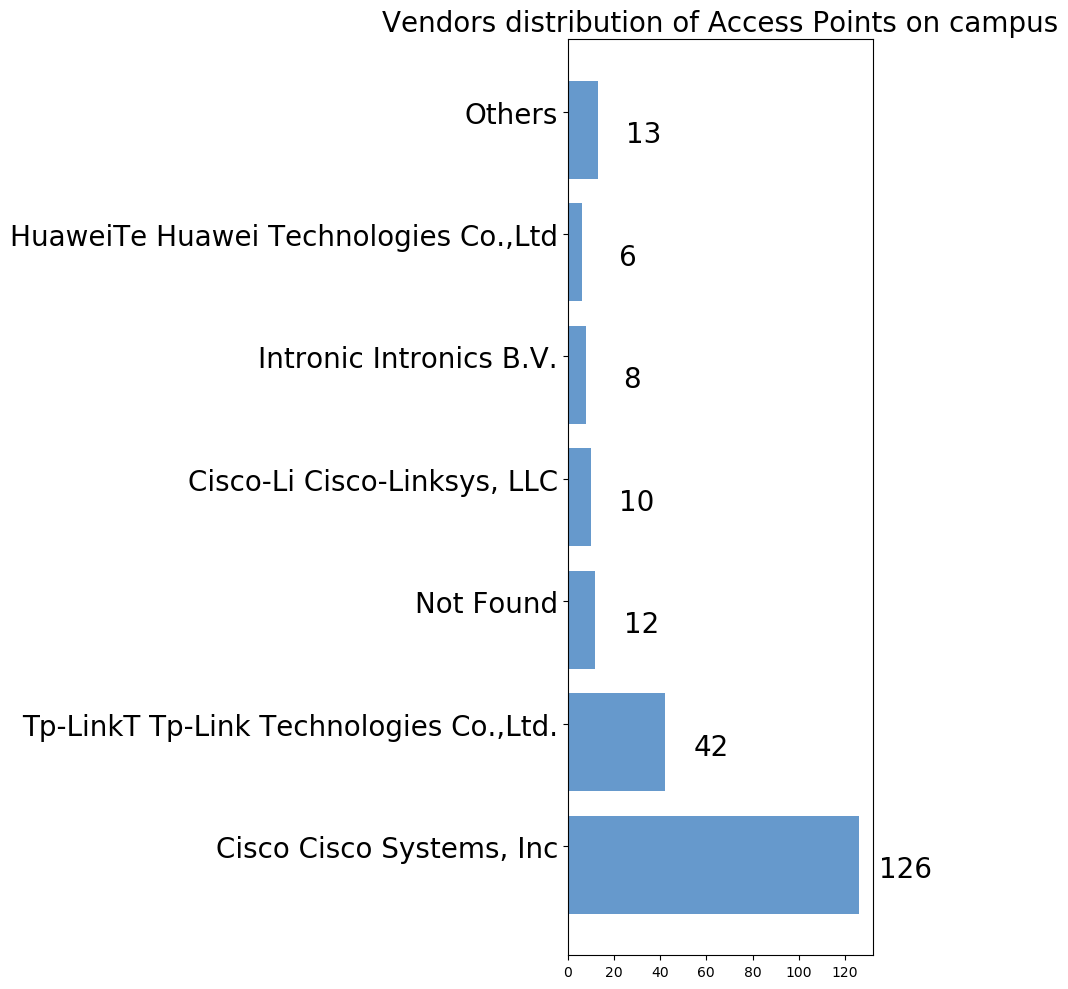
\includegraphics[width=1.5in,height=5cm]{Figure/Vendors distribution of Access Points on campus_bar.png}
    }
    \subfigure[Stations on campus]{
	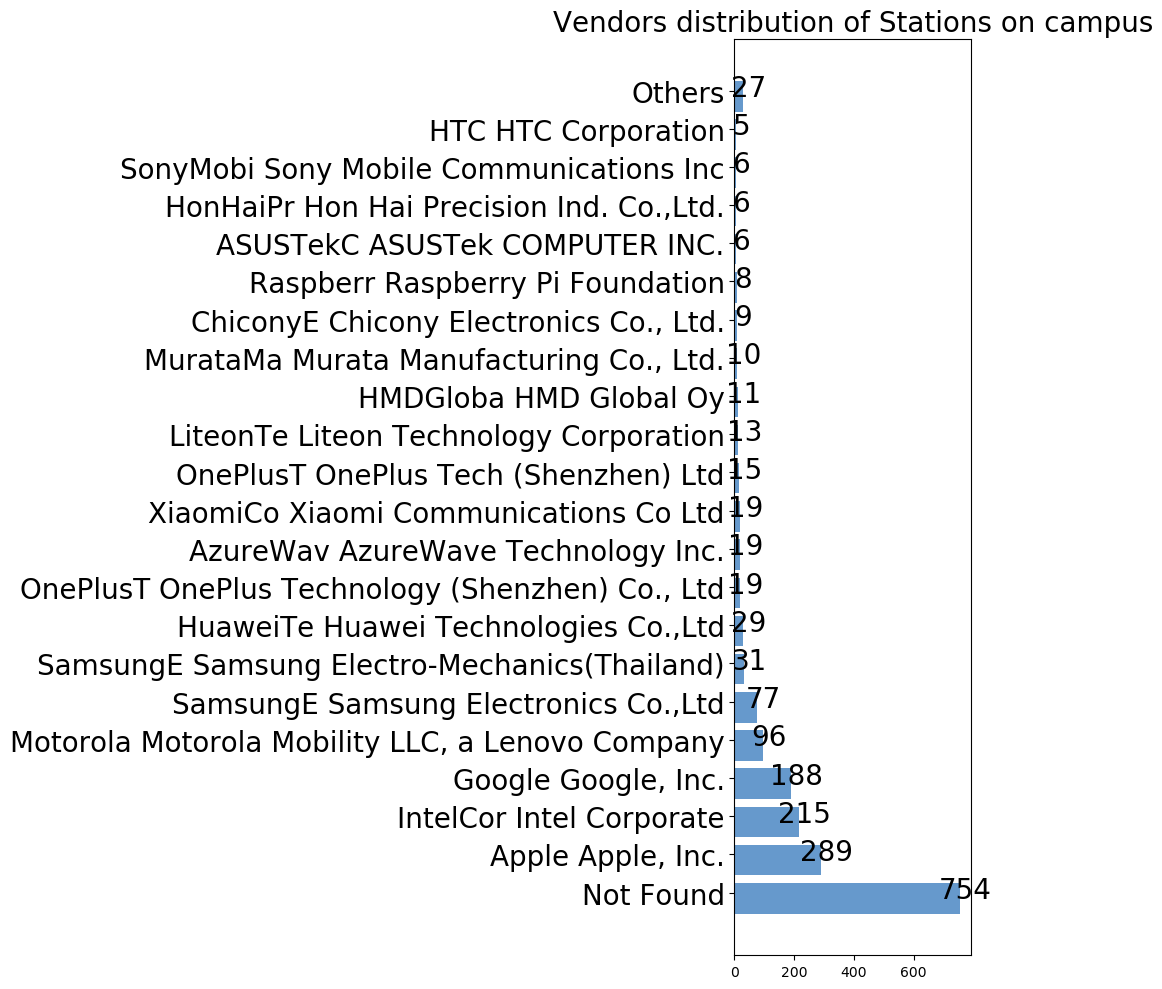
\includegraphics[width=1.5in,height=5cm]{Figure/Vendors distribution of Stations on campus_bar.png}
    }
    \quad   
    \subfigure[Access points near Roland Holstlaan]{
    	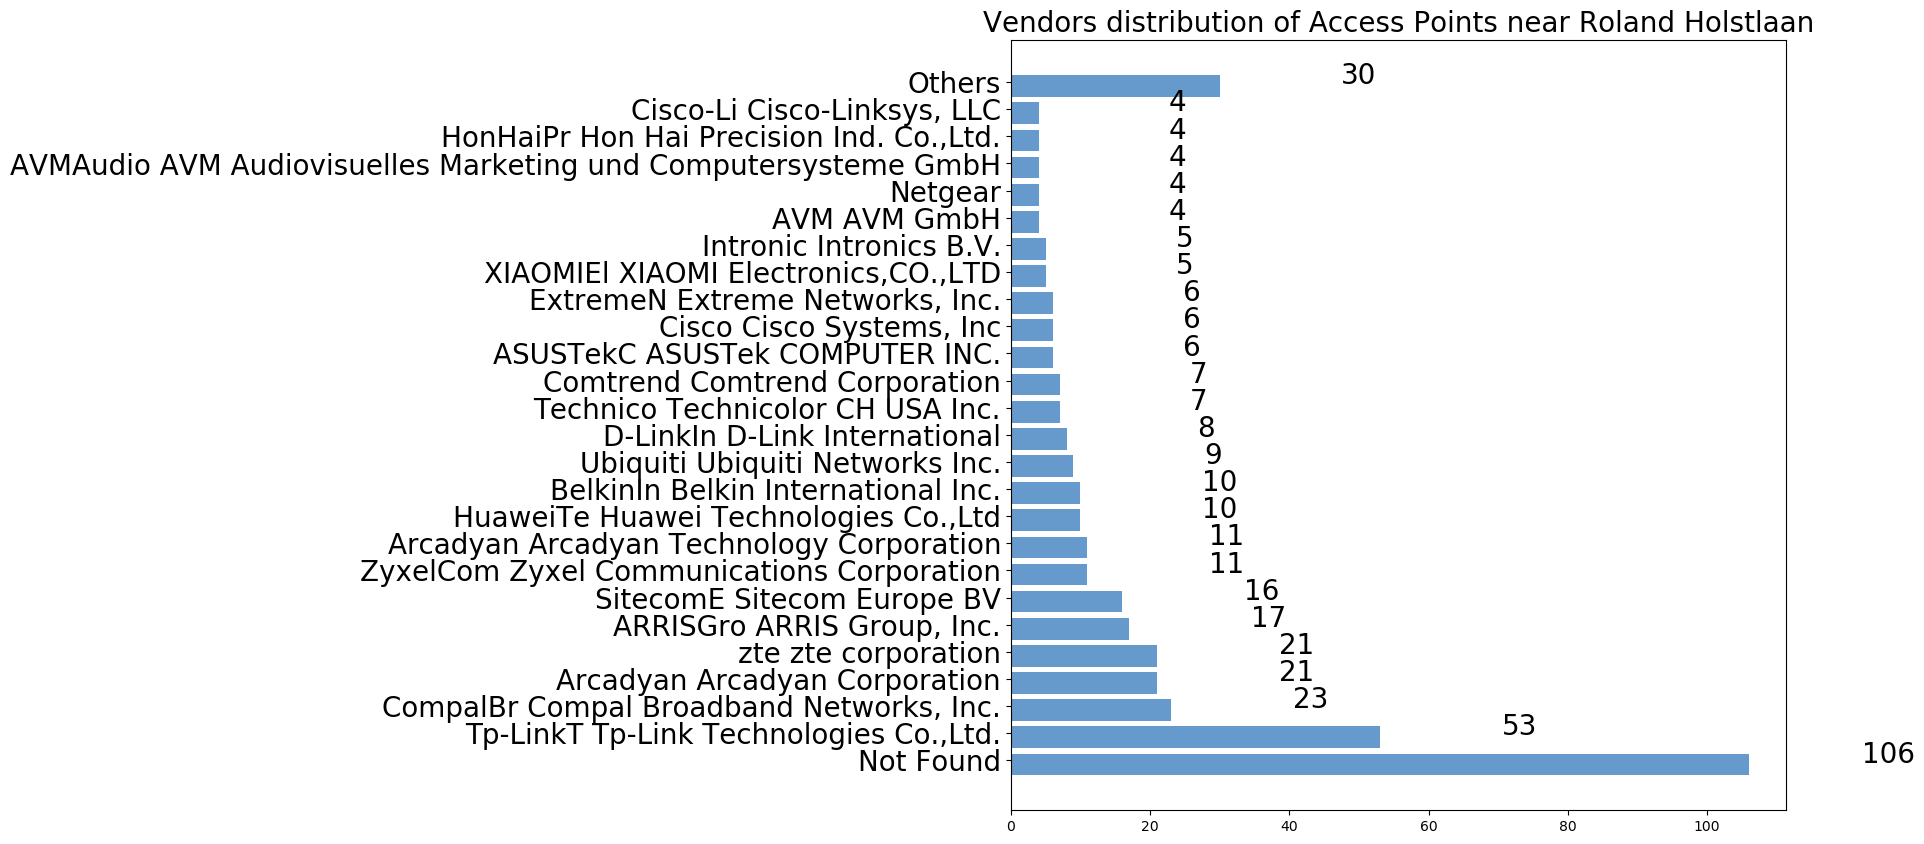
\includegraphics[width=1.5in,height=5cm]{Figure/Vendors distribution of Access Points near Roland Holstlaan_bar.png}
    }
    \subfigure[Stations near Roland Holstlaan]{
	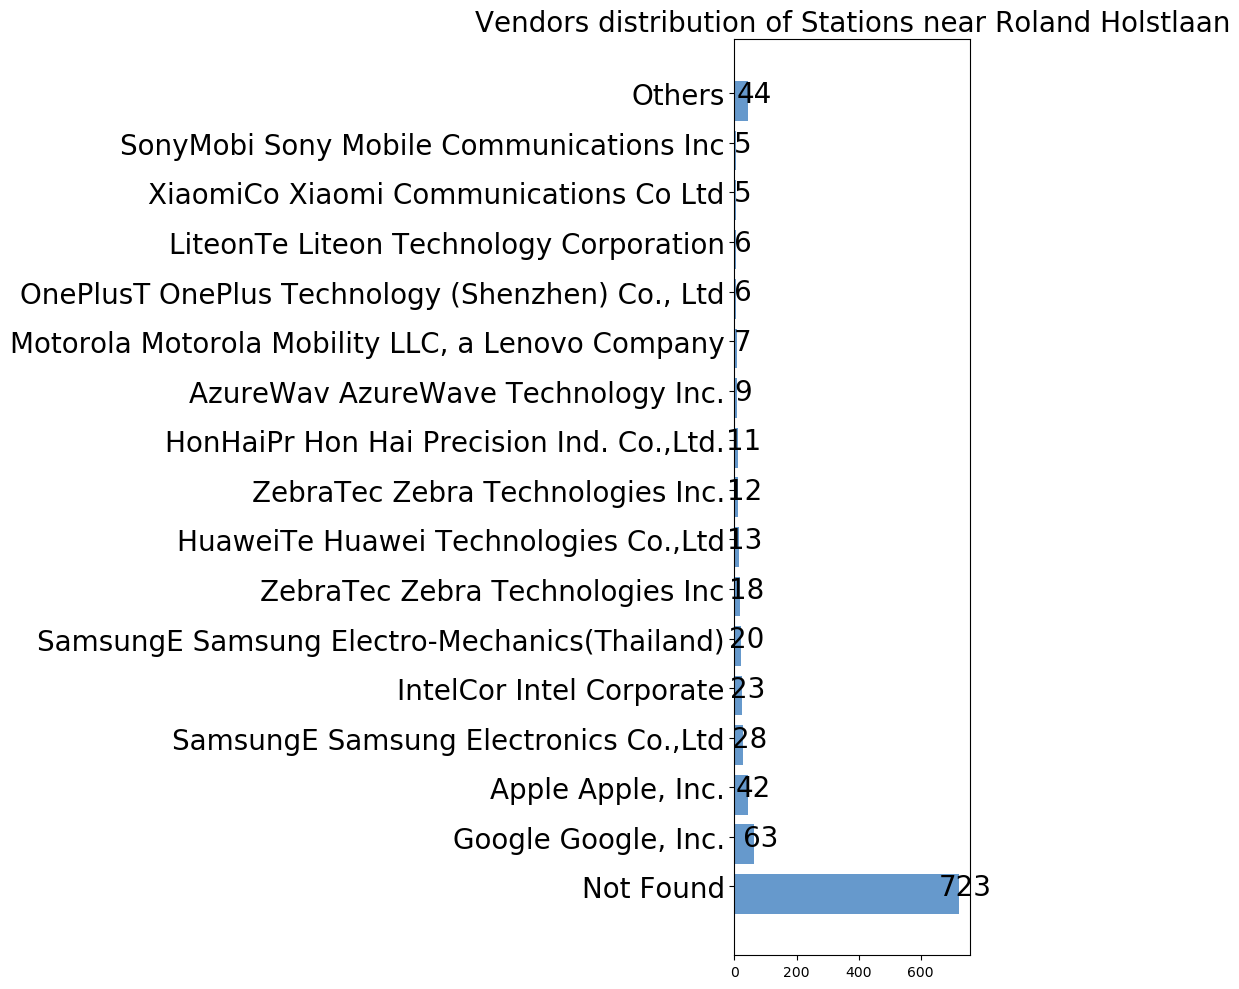
\includegraphics[width=1.5in,height=5cm]{Figure/Vendors distribution of Stations near Roland Holstlaan_bar.png}
    }
    \quad
        \subfigure[Access points near Hendrick de Keyserweg]{
    	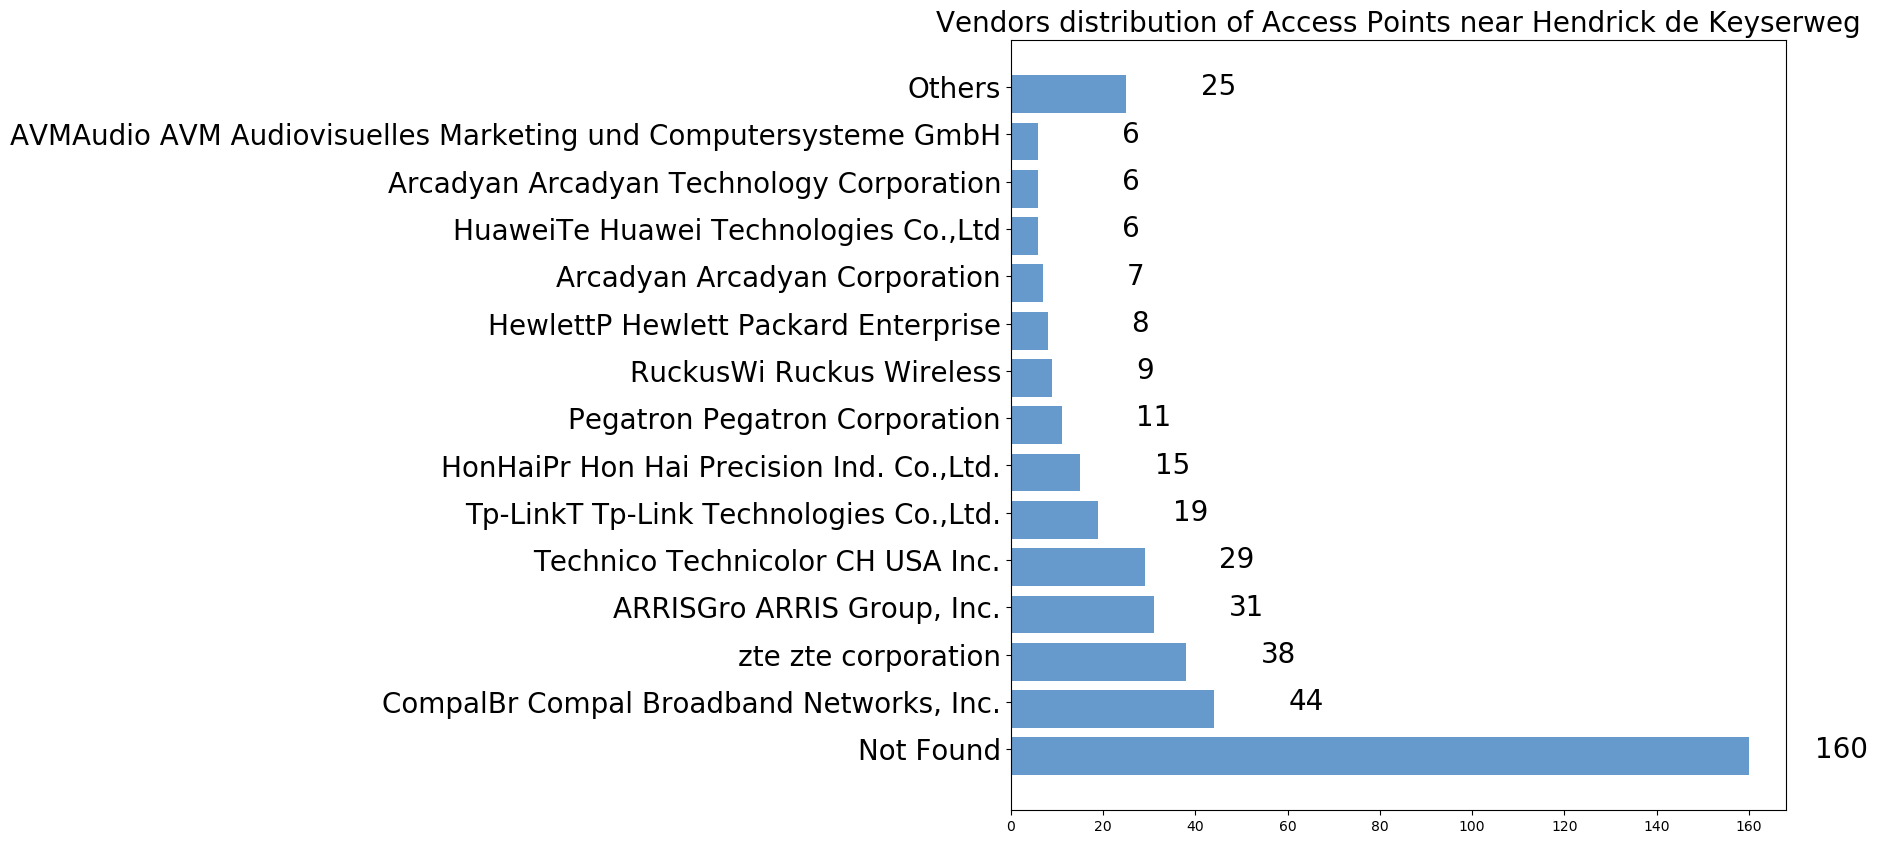
\includegraphics[width=1.5in,height=5cm]{Figure/Vendors distribution of Access Points near Hendrick de Keyserweg_bar.png}
    }
    \subfigure[Stations near Hendrick de Keyserweg]{
	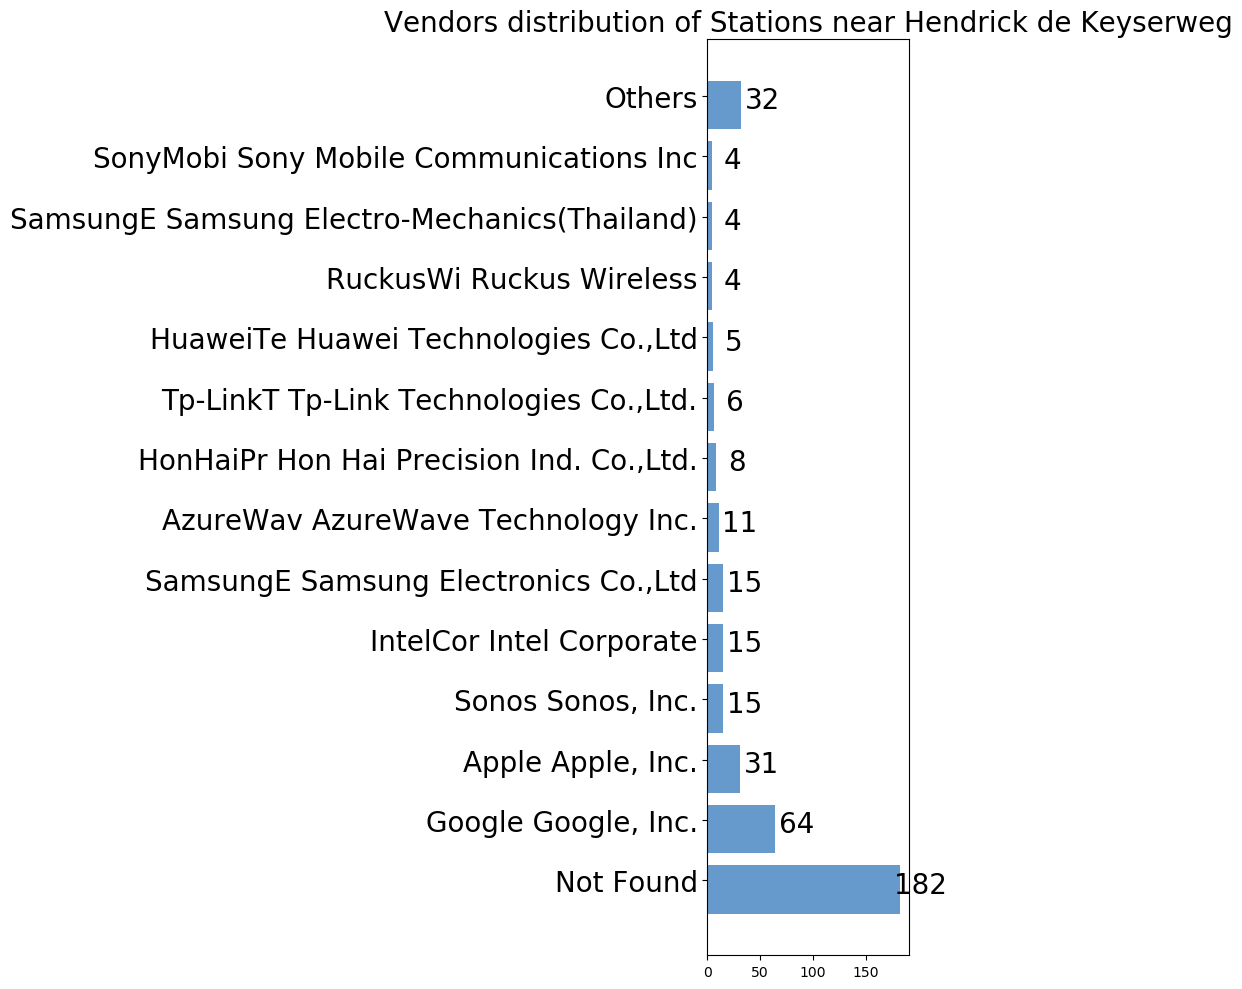
\includegraphics[width=1.5in,height=5cm]{Figure/Vendors distribution of Stations near Hendrick de Keyserweg_bar.png}
    }
    \caption{Vendors distribution of Access points(left) and stations(right)}
    \label{fig.1}
\end{figure}


\begin{figure}[H]
    \centering
    \subfigure{
        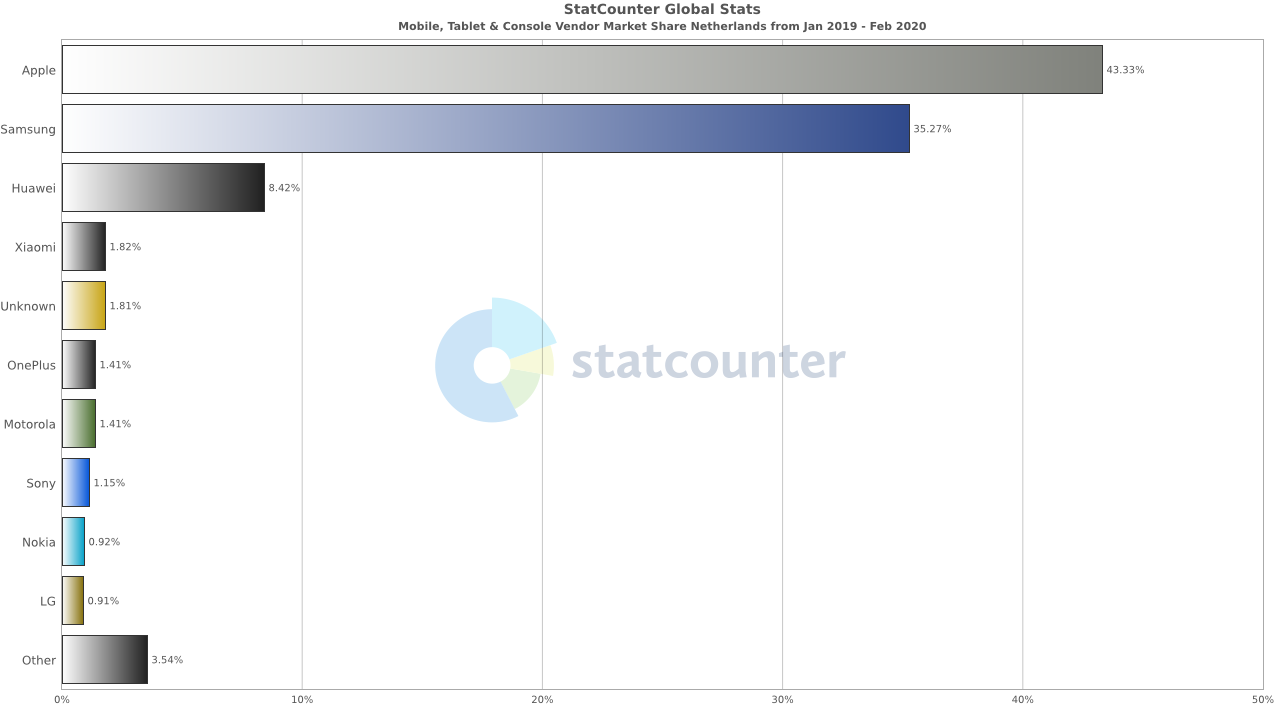
\includegraphics[width=3in]{Figure/Station distribution.png}
    }
    \caption{Vendors distribution of Netherlands from Jan 2019 to Feb 2020}
    \label{fig.2}
\end{figure}

\newpage
\begin{figure}[H]
    \centering
    \subfigure[Access points on campus]{
        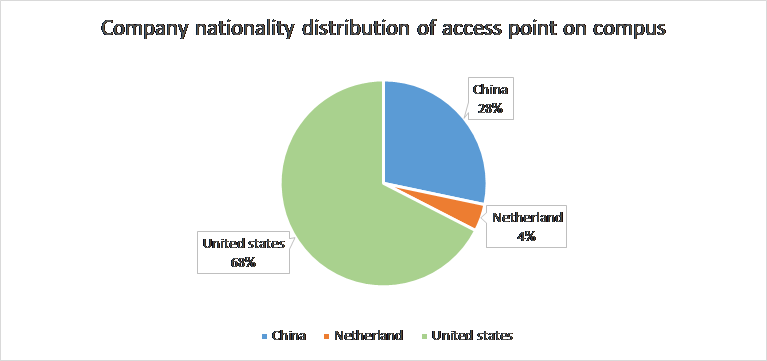
\includegraphics[width=1.5in]{Figure/piechart-ap-cam.png}
    }
    \subfigure[Stations on campus]{
	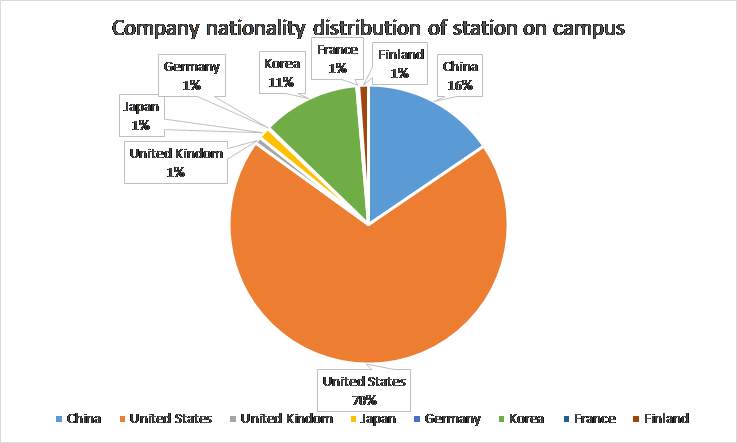
\includegraphics[width=1.5in]{Figure/Piechart-s-cam.png}
    }
    \quad   
    \subfigure[Access points near Roland Holstlaan]{
    	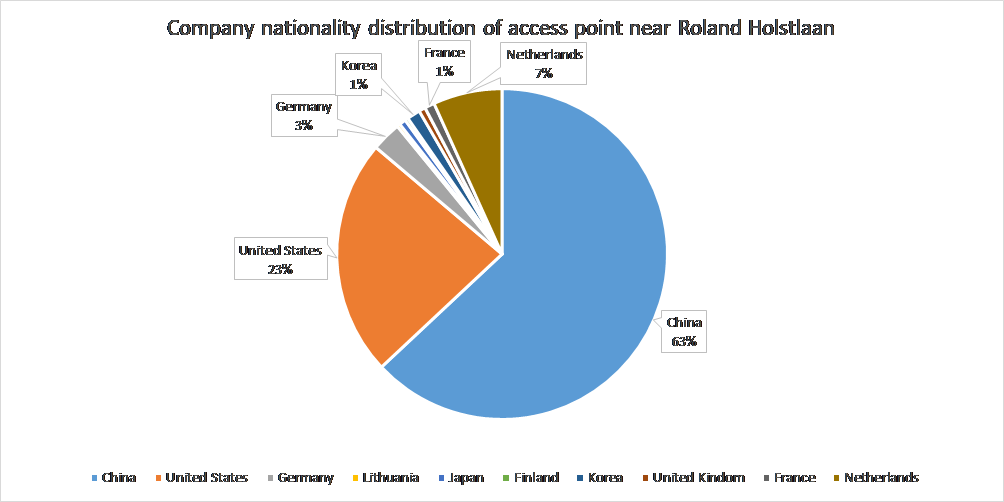
\includegraphics[width=1.5in]{Figure/piechart-ap-rh.png}
    }
    \subfigure[Stations near Roland Holstlaan]{
	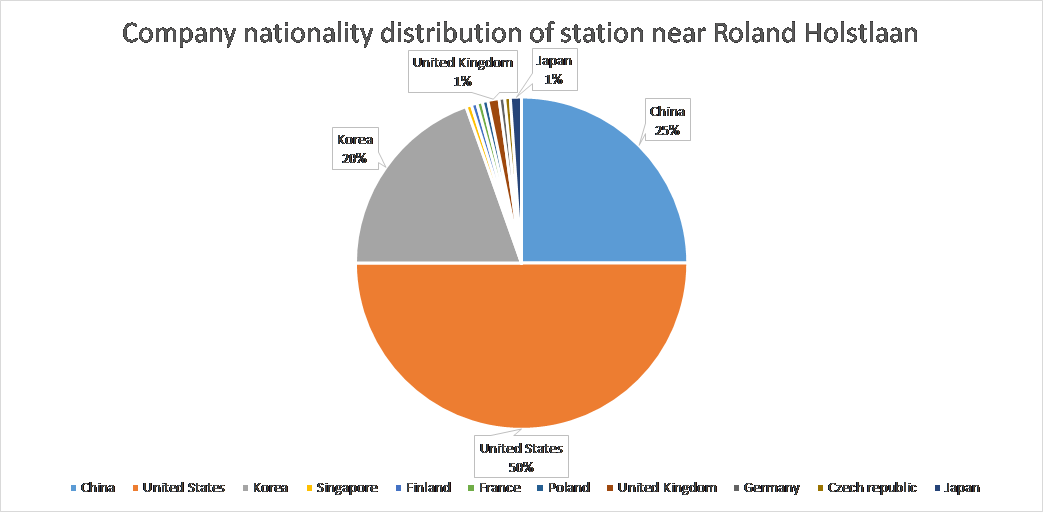
\includegraphics[width=1.5in]{Figure/piechart-s-rh.png}
    }
    \quad
        \subfigure[Access points near Hendrick de Keyserweg]{
    	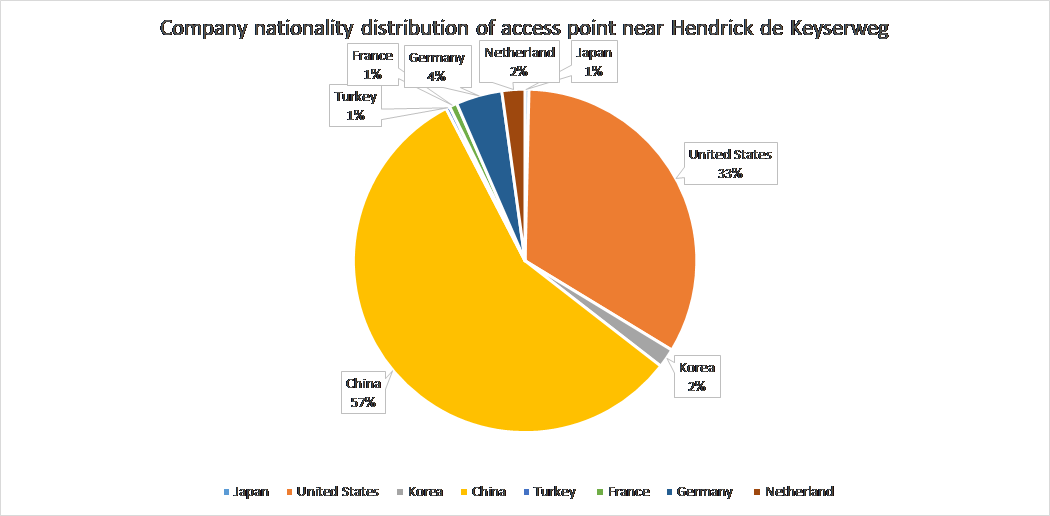
\includegraphics[width=1.5in]{Figure/piechart-ap-hk.png}
    }
    \subfigure[Stations near Hendrick de Keyserweg]{
	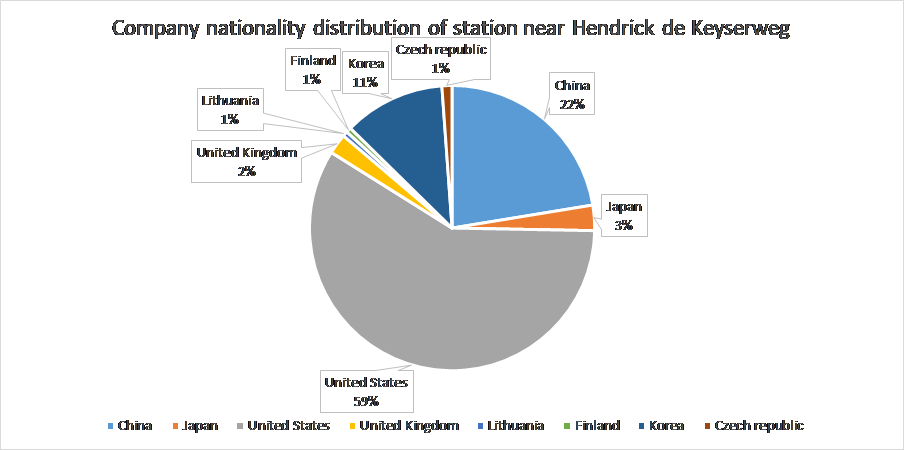
\includegraphics[width=1.5in]{Figure/piechart-s-hk.png}
    }

    \caption{Vendors nationality distribution of Access Points(left) and Stations(right)}
    \label{fig.3}
\end{figure}

Figure 3 shows the nationality information of vendors both in access point and station, from the pie chart, American and Chinese vendors account for a significant proportion for both access points and stations with others such as France, Germany, Turkey or the republic of Czech accounting for less than 10 percentages. For access points, Dutch vendors have a percentage in each of the three regions while vendors of other countries only have one or two percent. For the station, the Korean vendors have exhibited a more obvious ratio and even in the Roland dormitory area South Korea's ratio and China's ratio are all about 20 percent. This means South Korea still leads the market in the production of mobile devices.